\renewcommand{\chaptername}{Sistemas de coordenadas astronómicas}
\graphicspath{{parte_3/sist_coord/}}
\chapter{Sistemas de coordenadas astronómicas} \label{cap:sist_cord} 
\markright{Sistemas de coordenadas astronómicas} 
\begin{center}
	\begin{tcolorbox}[colback=gray!5!white, %Color del fondo
		colframe=blue!75!black,
		title= \center{\Large{Resumen}} ]
	Se brindan los fundamentos de las coordenadas astronómicas. Además, se resumen algunos de los sistemas de coordenadas utilizados en astronomía. Esta descripción es necesaria, para poder realizar la transformación de coordenadas dentro del microcontrolador, en caso que se este siguiendo una estrella o satélite,mediante el programa Stellarium,
	\end{tcolorbox}
\end{center}    

\section{introducción} 

En este capítulo se describe como realizar la transformación de coordenadas. El microcontrolador, recibe las coordenadas en coordenadas ecuatoriales horarias(con el software Stellarium), y debe realizar la transformación a coordenadas a ecuatoriales locales, luego debe realizarse otra transformación, al sistema horizontal local, dado el tipo de montura(altazimutal) que posee la antena. El presente capítulo, intenta explicar algunos de los sistemas de coordenadas se usan en astronomía, y necesarios para el presente trabajo. Existen más sistemas de coordenadas, pero rebasan el alcance del proyecto, el lector interesado puede ver la referencia \cite{Baume2014}. Antes de comprender los sistemas de coordenadas astronómicos, se debe empezar conociendo conceptos básicos de la trigonometría esférica, esfera celeste, etc. Al lector que este familiarizado con estos temas, puede omitir este capítulo. 

\section{Esfera - Elementos fundamentales} 


La superficie usada para las coordenadas astronómicas es la esfera. Por ello, se define una esfera, en conjunto con sus elementos fundamentales. A partir de esto, se obtienen algunos resultados de una materia denominada trigonometría esférica. Este tópico, plantea triángulos sobre la superficie de una esfera. Estos se arman a partir de los elementos básicos de una esfera. Por este motivo, la esfera se define a continuación: 

\begin{defin_esphere}
		 Conjunto de puntos del espacio equidistantes de otro punto fijo. 
\end{defin_esphere} 

Sobre esta definición, al punto fijo, se lo conoce como centro de la esfera y lo vamos a denotar con la letra \textbf{O}. La distancia desde O a cualquier punto, se denomina  \textbf{radio de la esfera (R)}  

Si a la esfera, se corta con un plano, según este plano contenga a O, o no, se definen dos tipos de círculos o circunferencias: 
\begin{itemize}
	\item \textbf{Circunferencia máxima (o circulo máximo)}: Circunferencia que se obtiene al cortar la esfera con el plano que contiene a \textbf{O}
	\item \textbf{Circunferencia menor (o circulo menor)}: Si el centro de la esfera(\textbf{O}) no esta contenida en el plano que corta a la esfera.
\end{itemize}

Ahora, para definir las posiciones de un punto, sobre la esfera, se requiere definir círculos de referencia, usando círculos menores y mayores. Si se tiene un círculo máximo, y se traza una recta perpendicular al plano del circulo máximo, y que pase por \textbf{O}, esta recta, corta a la esfera en dos puntos, denominados polos. Además de estos elementos, se tienen los siguientes: 
\begin{itemize}
	\item \textbf{Círculo fundamental}: circulo máximo mencionado. 
	\item \textbf{Círculos paralelos}: círculos paralelos al fundamental. Son círculos menores. 
	\item \textbf{Círculos secundarios}: círculos máximos que pasan por los polos. 
\end{itemize}

La imagen que se muestra a continuación muestra todos estos círculos definidos en esta sección:
\begin{figure}[ht!]
	\centering
	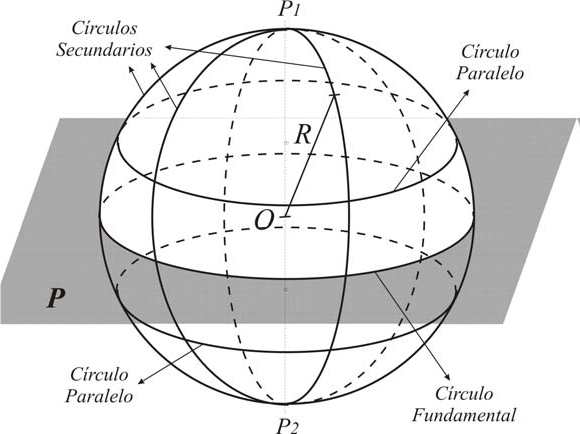
\includegraphics[scale=0.7]{circulos_fundamentales} 
	\caption{Esfera con sus elementos fundamentales}
	\label{fig:circ_fund}
\end{figure}

\section{Arcos y ángulos sobre una esfera} 

Se tiene que dados dos puntos A y P sobre una esfera, que no sean extremos de un diámetro, corresponden a un único circulo máximo o circunferencia máxima (figura \ref{fig:segAP}). La distancia más corta entre A y P es el arco de circunferencia AP 

Si ponemos otro punto, denominado B (ver figura \ref{fig:seg_ap_oa}), entonces, el circulo máximo entre B y P también es único. Este círculo, interseca al círculo máximo entre A y P, formando un ángulo $\alpha$, este ángulo, se denomina ``ángulo esférico'', y el punto de intersección se denomina vértice del ángulo esférico(P). El valor de este ángulo viene dado por el ángulo de intersección de los planos que contienen a los círculos máximos($\alpha$ en la figura \ref{fig:seg_ap_oa}).  

Si ahora se tienen dos arcos PA y PB, ambos siendo un cuarto de la circunferencia máxima, se tiene que el arco AB es igual al arco formado por la recta OA y OB (ver figura \ref{fig:triang_esfer_form}). Además, la longitud de la circunferencia es R$\alpha$. Así, para una esfera dada, la longitud del arco AB es proporcional a $\alpha$. Por ser el arco AB proporcional al radio, puede darse una unidad angular, o puede decirse que el radio de la esfera es uno, ya que en la esfera celeste el radio es desconocido(ver sección \ref{sec:esfera_celeste} distancia al objeto).  

\begin{figure}[ht]
	\centering
	
	\begin{subfigure}[t]{0.3\textwidth}
		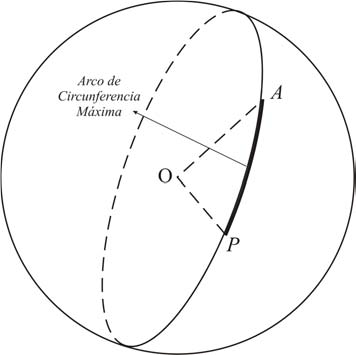
\includegraphics[width=\textwidth]{segmento_ap1} 
		\caption{Segmento AP sobre una esfera}	
		\label{fig:segAP}
	\end{subfigure}
	\hfill
	\begin{subfigure}[t]{0.3\textwidth}
		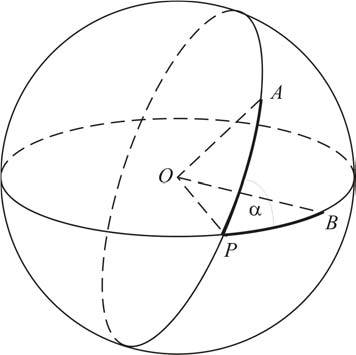
\includegraphics[width=\textwidth]{segmento_ap2} 
		\caption{Segmentos AP y OA sobre una esfera}	
		\label{fig:seg_ap_oa}	
	\end{subfigure}
	\hfill
	\begin{subfigure}[t]{0.3\textwidth}
		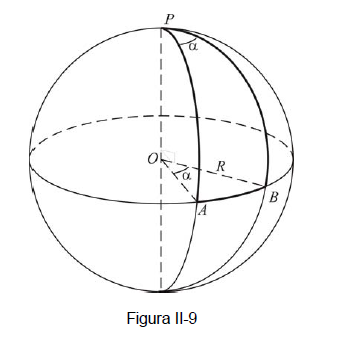
\includegraphics[trim={0 1.2cm 0 0},clip=true,width=1.3\textwidth]{segmento_ap3} 
		\caption{Formación de un triángulo esférico}		
		\label{fig:triang_esfer_form}
	\end{subfigure}
	
	\caption{Ubicación de puntos sobre una esfera}
\end{figure}

\section{Trigonometría esférica} 

La trigonometría esférica es una parte de la geometría esférica que estudia los triángulos formados por en la superficie de una esfera. Este tópico, es de importancia para comprender los sistemas de coordenadas empleados, y obtener las relaciones entre ellos. Así como en la geometría plana, existen los teoremas del coseno y del seno, aquí se obtiene algo similar, con el mismo nombre, además, a partir de estos, se obtiene la denominada ``formula de los cinco elementos''. 


Para comenzar, se debe realizar un triángulo esférico. Este triangulo esférico, se forma por la intersección de tres planos de circulo máximo con una esfera. Esta intersección forma un triángulo sobre la superficie de la esfera. Este triangulo, está determinado por tres arcos de circunferencia. Los elementos de este triangulo son los tres arcos, y los tres ángulos diedros entre ellos. Por convención denotamos los arcos con minúscula y los vértices con mayúscula. Así, el vértice A, tiene por opuesto el arco a, y así sucesivamente. En la siguiente figura se observa la formación un triángulo esférico. 
%El triángulo esférico y su formación se observa en la figura \ref{fig:form_triang_esfer}

\begin{figure}[ht]
	\centering
	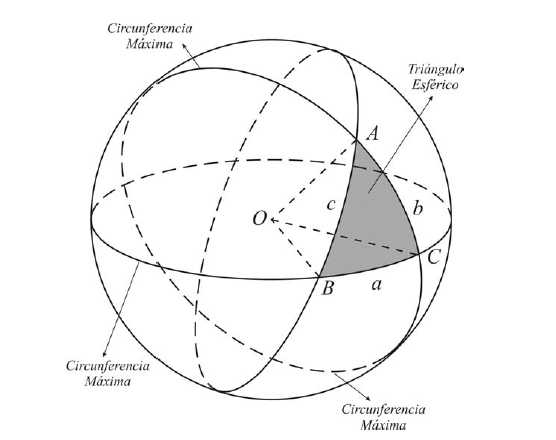
\includegraphics[scale=0.5]{triang_esfer_5_el}
	\caption{Formación de un triángulo esférico. Se muestran los lados principales y la intersección de tres planos para formarlo.}
	\label{fig:form_triang_esfer}
\end{figure}
\vspace{-5mm}
Para obtener las relaciones entre los ángulos y lados del triángulo esférico, se toma el triángulo y se aísla, luego realiza la siguiente construcción geométrica: se dibuja la recta tangente al segmento b en el punto A, y otra recta tangente en el arco c en el punto A. La recta tangente se extiende hasta el plano definido por ODE. Este procedimiento se observa en la figura \ref{fig:triang_aisl}. 
\begin{figure}[ht!]
	\centering
	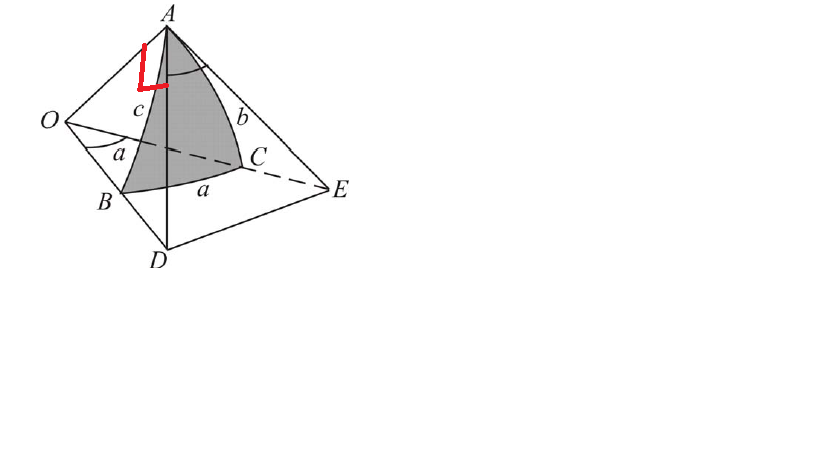
\includegraphics[trim={0 5cm 8cm 0},clip=true]{triang_esfer_aisl} 
	\caption{Triángulo esférico aislado. En rojo se muestra el ángulo recto.}
	\label{fig:triang_aisl}
\end{figure}
En la figura \ref{fig:triang_aisl}, segmento AD es tangente al arco c, y el segmento AE es tangente al arco b. Debido a que el segmento OAB y OAC son círculos, sus tangentes son perpendiculares a la recta que une sus centros. Es decir, los ángulos formados por OAD y OAE tienen 90°. Además, notamos que el ángulo DOE es el arco $a$ (o arco BC), y por definición, DAE es el ángulo esférico en A. A partir de esto, se usa el teorema del coseno para triángulos planos, y se tiene una especie de pirámide con cuatro triángulos. 


\subsection{Teorema del coseno para triángulos esféricos}
A partir de la figura \ref{fig:triang_aisl} se obtiene la siguiente relación de los tríangulos DOE y DAE. A partir del teorema del coseno para triángulos, se tiene: 
%\begin{equation}
\begin{align}
	\overline{DE}^2 & = \overline{OD}^2+\overline{OE}^2-2\overline{OD} \ \overline{OE} \cos(\widehat{DOE})\annoterel{$\widehat{DOE}=a$(ver figura \ref{fig:triang_aisl})}{=} \overline{OD}^2+\overline{OE}^2-2\overline{OD} \ \overline{OE} \cos(a)  \\
\overline{DE}^2 & = \overline{AD}^2+\overline{AE}^2 - 2\overline{AD} \ \overline{AE} \cos(A) 
\end{align}
%\end{equation}

Donde la primera expresión corresponde al triángulo $\overline{DOE}$ y la segunda al triángulo $\overline{DAE}$.Igualando las expresiones anteriores, y operando algebraicamente, se obtiene la siguiente expresión: 

\begin{equation} \label{eq:tri_esf1}
	(\overline{OD}^2 - \overline{AD}^2) + (\overline{OE}^2 - \overline{AE}^2) = 2(\overline{OD}\ \overline{OE}\cos(a)+ \overline{AD}\ \overline{AE}\cos(A) )
\end{equation}

Por lo expuesto en la sección anterior, los triángulos $\overline{DOA}$ y $\overline{OEA}$
son triangulos rectángulos. Se usa el teorema de Pitágoras aplicado al triángulo $\overline{DOA}$  y se obtiene que $\overline{OD}^2=\overline{OA}^2 + \overline{AD}^2$. Del mismo modo, se aplica el teorema al triángulo rectángulo $\overline{OEA}$, y se obtiene $\overline{OE}^2=\overline{OA}^2 + \overline{AE}^2$. De estas expresiones, podemos obtener expresiones para el miembro izquierdo de la igualdad de la ecuación \ref{eq:tri_esf1}. La suma de ambos miembros, da por resultado $2\overline{OA}$, y reemplazando resulta en la siguiente expresión: 
\begin{equation} \label{eq:tri2_esf}
	\overline{OA}^2 = (\overline{OD}\ \overline{OE}\cos(a)+ \overline{AD}\ \overline{AE}\cos(A) )
\end{equation}   

Como los triángulos que se observan($\overline{OEA}$ y $\overline{ODA}$), son rectángulos en A. Por medio de esta observación, se obtienen expresiones para $\overline{OD}$, $\overline{OE}$, y $\overline{AD}$ y $\overline{AE}$. Estas se obtienen usando relaciones trigonométricas(seno y coseno). El ángulo entre EOA es b, ídem si miramos otros ángulos. Con esta observación, se obtienen las siguientes relaciones:
 

\begin{equation}
	\cos(b) =  \frac{\overline{OA}}{\overline{OE}} \qquad \sin(b) = \frac{\overline{AE}}{\overline{OE}} \qquad
	\cos(c) = \frac{\overline{OA}}{\overline{OD}} \qquad
	\sin(C) = \frac{\overline{AD}}{\overline{OD}} 
\end{equation}

Reemplazando estas expresiones, en la ecuación \ref{eq:tri2_esf}. Luego, de realizar este reemplazo, se despeja de la expresión resultante $\cos(a)$, se obtiene una de las ecuaciones referidas a la ley del coseno esférico.
\begin{equation}
	\cos(a) = \cos(b)\cos(c) + \sin(c)\sin(b)\cos(A) 
\end{equation}

Realizando este procedimiento, sobre todos los triángulos de la figura \ref{fig:triang_aisl}, se obtiene \textbf{la ley del coseno para triángulos esféricos}: 

\begin{equation} \label{eq:ley_cos_esf}
\left\{\begin{array}{c} 
	\cos(a) = \cos(b)\cos(c) + \sin(c)\sin(b)\cos(A) \\ 
	\cos(b) = \cos(a)\cos(c) + \sin(a)\sin(c)\cos(B) \\	
	\cos(c) = \cos(a) \cos(b) + \sin(a) \sin(b) \cos(C)
\end{array} \right.  
\end{equation}

\subsection{Ley del seno para triángulos esféricos}

Esta ley establece las relaciones entre ángulos diedros, y segmentos angulares del triángulo esférico. Para demostrar su validez, se parte de la expresión de la ley de los cosenos. Si tomamos la primera expresión de la ley de los cosenos(ecuación \ref{eq:ley_cos_esf}), y despejamos en términos de los senos, se obtiene lo siguiente: 

\begin{equation*}
	\sin(b) \sin(c)\cos(A)=\cos(a)-\cos(b)  \cos(c)	
\end{equation*}

De la expresión anterior, elevando ambos miembros al cuadrado, y operando algebraicamente, usando identidades trigonométricas, se llega a la siguiente expresión: 

\begin{equation}
	\sin^2(b)\sin^2(c)\sin^2(A) = 1 - \cos^2(a) - \cos^2(b)-\cos^2(c) + 2\cos(a) \cos(b) \cos(c)
\end{equation}

%En la expresión anterior, del lado derecho de la igualdad, se observa que la expresión no depende de A.
Si se realiza el mismo procedimiento para cada ecuación de la ley de cosenos esféricos, se obtiene la misma expresión, para las otras dos ecuaciones. Luego, se igualan las tres expresiones, queda: 

\begin{equation*}
	\sin^2(b)\sin^2(c)\sin^2(A) = \sin^2(b)\sin^2(c)\sin^2(C) = \sin^2(a)\sin^2(c)\sin^2(B)   
\end{equation*}

Dividiendo ambos miembros por la expresión $\sin^2(a)\sin^2(b)\sin^2(c)$(esto se puede realizar, dado que todos los ángulos oscilan entre 0$^\circ$ y 180$^\circ$). Luego, se toma en todos los miembros, raiz cuadrada, se obtiene la siguiente expresión: 

\begin{equation}
	\frac{\sin(A)}{\sin(a)} = \frac{\sin(C)}{\sin(c)} = \frac{\sin(B)}{\sin(b)}   
\end{equation}  

Esta expresión, se denomina \textbf{Ley del seno para triángulos esféricos}.


\section{Fórmula de los cinco elementos} 

La ley del coseno para triángulos esféricos, como la ley del seno, contemplan solo cuatro elementos del triángulo esférico. Utilizando la ley del coseno, puede obtenerse un grupo de seis(6) formulas, para tener una expresión que contemple cinco elementos del triángulo esférico. Se parte de la primera ecuación de la ley del coseno (ecuación \ref{eq:ley_cos_esf}), y se obtiene lo siguiente: 
\begin{equation}
	\sin(b)\sin(c)\cos(A) = \cos(a) - \cos(b)\cos(c) 
\end{equation} 

Del conjunto de ecuaciones \ref{eq:ley_cos_esf}, se toma la tercera ecuación($\cos(c)$), y se reemplaza en la expresión anterior, realizando este paso, se obtiene la siguiente expresión: 

\begin{equation}
	\sin(b)\sin(c)\cos(A) = \cos(a)\sin^2(b) - \cos(b)\sin(a)\sin(b)\cos(C) 
\end{equation}

Se divide ambos miembros de la expresión anterior por $\sin(b)$, se obtiene la primera expresión que vincula cinco elementos del triángulo esférico: 

\begin{equation}
	\sin(b)\cos(A) = \cos(a)\sin(b) - \cos(b)\sin(a)\cos(C) 
\end{equation}

La ecuación anterior, representa la \textbf{fórmula de los cinco elementos para triángulos esféricos} 

Se observa, en la expresión anterior, que esta expresión, relaciona cinco elementos del triángulo esférico. Realizando un procedimiento similar, se obtiene un conjunto de 6 ecuaciones, que relacionan todos los elementos. Estas expresiones vienen dadas por: 
%\begin{equation}
\begin{align}
	\begin{cases}	
		\sin(c)\cos(A) = \cos(a)\cos(b) - \cos(b) \sin(a) \cos(C) \\
		\sin(c)\cos(B) = \cos(b)\sin(b) - \cos(a) \sin(b) \cos(C) 	
	\end{cases}
    \\
	\begin{cases}
		\sin(b)\cos(A) = \cos(a)\sin(c) - \sin(a) \cos(c) \cos(B) \\
		\sin(b)\cos(C) = \cos(c)\sin(a) - \sin(c) \cos(a) \cos(B) 	
    \end{cases}
	\\
	\begin{cases}
		\sin(a)\cos(B) = \cos(b)\sin(c) - \sin(b) \cos(c) \cos(A) \\
		\sin(a)\cos(C) = \cos(c)\sin(b) - \sin(c) \cos(b) \cos(A) 	
	\end{cases}
\end{align}


\section{Ubicación de los puntos sobre una esfera} 



En este punto, se describe como realizar la medición de los puntos sobre una esfera. El sistema utilizado es el sistema de coordenadas esféricas. Este sistema, solo requiere de dos coordenadas angulares para ubicar un punto sobre la superficie (esto es así, porque el radio de una esfera permanece constante). La figura \ref{fig:ubic_point_sphere}, muestra dos arcos de circunferencia, los cuales son CB y BA. Luego, para obtener las coordenadas del punto A, se debe girar un ángulo CB, y otro ángulo BA. Este par ordenado da la posición del punto A. Además, se debe elegir un origen para el sistema de coordenadas esférico del cual se toma como ángulo cero. En la imagen \ref{fig:ubic_point_sphere} es el punto C, sobre un círculo máximo. A partir de este círculo, se define otra medida angular, el arco BA, medido desde el plano que pasa por el origen y contiene a C. En otras palabras, el ángulo BA, se mide sobre el circulo secundario, tomando como ángulo cero, el punto B. Si este ángulo se define negativo o positivo, o de 0º a 360º, depende de la aplicación particular.  

\begin{figure}[ht!]
	\centering
	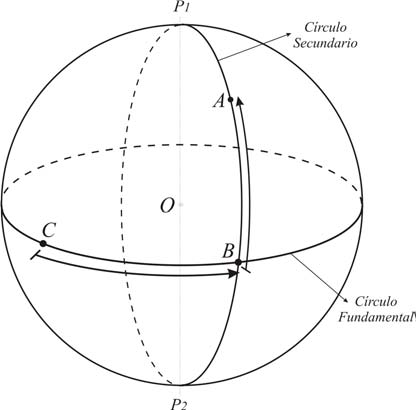
\includegraphics{ubicacion_esfera_point} 
	\caption{Ubicación de un punto usando un plano de referencia}
	\label{fig:ubic_point_sphere}
\end{figure}


\section{La esfera Celeste} \label{sec:esfera_celeste}

Una vez, conocidas las partes fundamentales de una esfera, se debe conocer una esfera que es de importancia en astronomía de posición, la esfera celeste. Esta esfera, se compone de un centro O, denominado centro de observación. En el centro, se ubica el observador de los astros, o satélites en nuestro caso. Cabe recalcar, que esta esfera es una construcción ficticia para determinar la posición de los astros, es decir, es una abstracción para poder ubicar objetos en el cielo. 
La observación astronómica, depende de la posición del observador sobre el planeta tierra, por este motivo, se debe conocer los puntos de la tierra, su sistema de coordenadas, para poder determinar la orientación de una antena o telescopio. Estos sistemas de coordenadas son latitud y longitud, y se requiere de una definición formal, ya que a partir de estos, se realiza la transformación de coordenadas. 

\section{Elementos de la superficie terrestre y Sistemas de coordenadas geográficos}

Él seguimiento de las estrellas, astros y satélites, dependen de la posición del observador en la superficie terrestre. Al depender de la posición del observador sobre la superficie terrestre, se deben dar los datos de observación y la ubicación del observador. Esta ubicación, está dada por la latitud y la longitud del lugar y además, se requieren de otros planos, como el ecuador y el eje de rotación de la tierra. Es por este motivo, que la presente sección, se van a presentar los elementos fundamentales de la superficie terrestre. 

El planeta tierra posee una forma casi esférica. Existe una línea recta imaginaria sobre la cual gira el planeta tierra sobre su propio eje. Esta línea imaginaria, pasa por el centro de la tierra, y toca a la esfera en dos puntos: el polo norte geográfico (PNg) y el polo sur geográfico (PSg). El plano que es perpendicular a esta línea recta, se denomina ecuador terrestre. Este plano, divide a la tierra en dos hemisferios: hemisferio boreal (hemisferio norte) y hemisferio austral (hemisferio sur). Los planos paralelos al ecuador, que cortan al planeta tierra en círculos menores, se denominan paralelos geográficos. Existen cuatro de ellos con nombres particulares:

\begin{itemize}
	\item Trópico de cáncer 
	\item Trópico de Capricornio 
	\item Círculo polar Ártico. 
	\item Círculo polar Antártico. 
\end{itemize}

El semicírculo que pasa por los polos geográficos, y por un punto O de su superficie, se denomina meridiano geográfico del punto O. El meridiano que pasa por el observatorio de Greenwich (en Inglaterra), se denomina primer meridiano, o meridiano de grenwich. Este meridiano, junto con el que esta a 180° de él, divide a la tierra en otros dos hemisferios: hemisferio occidental y hemisferio oriental. El meridiano de Greenwich, se toma como cero. La siguiente imagen, aclara los conceptos explicados hasta aquí:
 
\begin{figure}[ht!]
	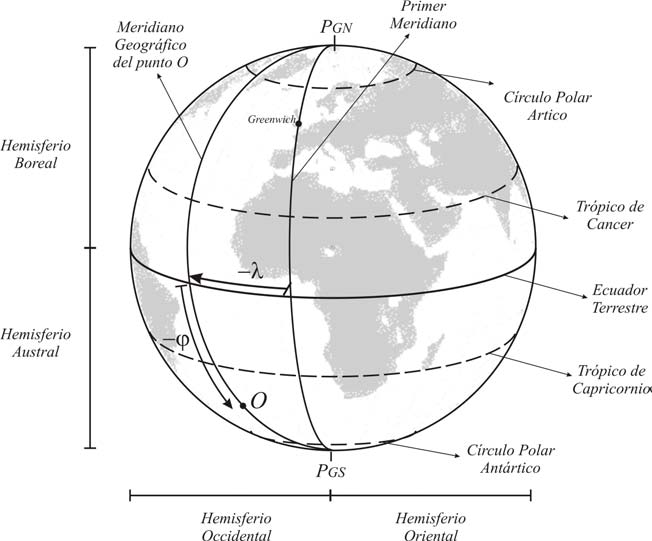
\includegraphics{coordenadas_terrestres}
	\caption{Tierra supuesta de forma esférica para mostrar sus elementos principales. Se muestran todos los datos necesarios para la ubicación de un punto sobre la superficie terrestre}
	\label{fig:coord_terr}
\end{figure}

Luego, se tienen las siguientes definiciones de latitud y longitud, con sus respectivos símbolos: 

\begin{itemize}
	\item \textbf{Longitud($\lambda$)}:Esta se mide desde la intersección del primer meridiano con el ecuador terrestre, hasta el circulo secundario que pasa por O. Este se mide, desde -180° a 180°, siendo el O, el cruce del meridiano de Greenwich con el ecuador. Si está en el hemisferio oriental, va de 0 a 180°, si se encuentra en el hemisferio occidental, va de -180° a 0°. Otra convención, es agregar la palabra “este u oeste”, y dar el valor de longitud en valor absoluto. Esta notación, no se emplea por ser confusa, y no se dirá más al respecto. 
	\item \textbf{Latitud($\phi$)}:se mide sobre el meridiano del punto O, desde el ecuador terrestre. Este valor oscila desde -90° a 90°. Los valores positivos corresponden al hemisferio boreal, y los negativos al hemisferio sur.
\end{itemize}


\section{Definición y elementos de la esfera celeste}
Si se encuentra en una zona despoblada, usted al observar el cielo, se tiene la impresión de encontrarse dentro de una esfera, la cual se ve únicamente la parte superior de ella. Esta idea es la que se usa para construir la esfera celeste. Esta esfera, puede tener su origen en tres puntos distintos, el primero, es el del observador, segundo, en el centro de la tierra, y el tercero, en el centro del sol. La que tiene el centro en la posición del observador, se denomina ``esfera celeste topocéntrica'', la que tiene su centro en la tierra, se denomina ``esfera celeste geocéntrica'' y la otra esfera es denominada ``heliocéntrica''. La diferencia entre ambas, es su origen de coordenadas. Estas difieren en algunos segundos de arco para observación, ya que la observación del cielo contiene otros fenómenos como difracción, paralaje, etc. Esta diferencia, se hace necesaria, cuando se trabaja con instrumentos que tengan la precisión para diferenciar estos segundos de arco.


Por lo visto en el párrafo anterior, se puede dar una definición formal de la esfera celeste: ``Esfera de radio unidad en cuyo centro(O) se encuentra el observador''. Cabe destacar, que la distancia del observador al astro es desconocida, por eso se elige de radio unidad. Además, al observar el cielo, este da la impresión de que todos los puntos se encuentran en la misma distancia. Una vez definida, la esfera celeste, en el presente trabajo usamos la esfera topocéntrica, ya que es la que toma al observador en la superficie terrestre.


La esfera celeste topocéntrica se muestra en la siguiente imagen(se muestra solo la parte superior): 

\begin{figure}[ht!]
	\centering
	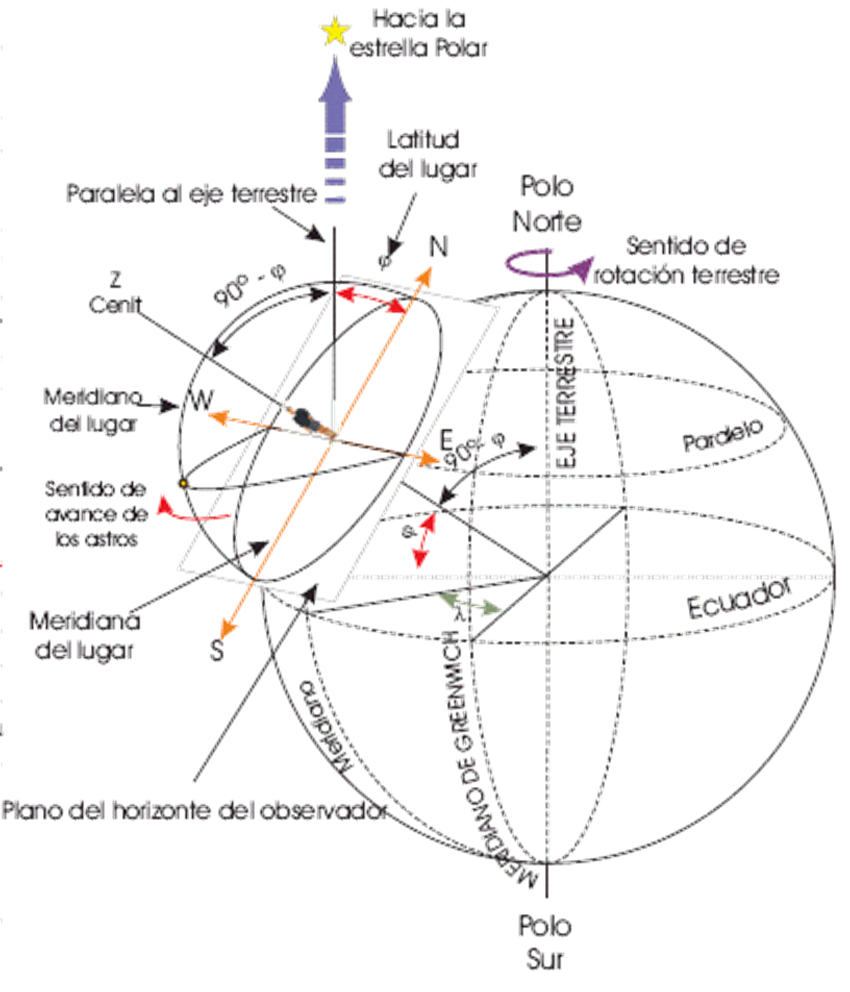
\includegraphics[scale=0.5]{esfera_celeste_topo}
	\caption{Esfera celeste ubicada en el plano del horizonte. En ella, se omite la parte no visible de la esfera celeste}
	\label{fig:esfera_celeste_topo}
\end{figure}


En el gráfico, se observa un plano de circulo máximo, que es tangente a la superficie terrestre, este plano se denomina ``plano del horizonte''. Este plano, al intersecarse con el meridiano del observador(longitud del observador), define la dirección Norte en este plano, y el Sur. En el gráfico aparecen con la letra N y S respectivamente. Además, este plano, divide a la esfera celeste en dos regiones ``horizonte visible'' y ``horizonte no visible''.En el gráfico se muestra el horizonte visible, el horizonte no visible, se encuentra debajo del observador. Si desde el lugar de observación, se lanza una plomada (dirección de la gravedad en ese punto), se observa que esta dirección, es perpendicular al plano del horizonte. Este plano, corta a la esfera celeste en dos puntos particulares: zenit y nadir. El zenit, se encuentra por encima del observador y a 90° del plano del horizonte. Este punto se encuentra en el horizonte visible. Se denota con z en la gráfica. El nadir no se encuentra dibujado. 

Esta esfera celeste, se encuentra rotando en torno a un eje: el eje de rotación de la tierra. Si tomamos el eje de rotación, de la tierra, y se translada de manera paralela a este mismo, obtenemos otro punto de la esfera celeste: el polo sur celeste y el polo norte celeste. En el gráfico se dibuja solo el polo norte celeste. Este eje, forma un ángulo con el zenit, que es $90 – \phi$ , o dicho de otra manera, si miro al norte sobre el meridiano, me elevo un angulo $\phi$, tengo un eje paralelo al eje de rotación terrestre. 


Si sobre el eje de rotación del polo sur celeste y del polo norte celeste, trazamos un círculo máximo, perpendicular a él, y que pase por el observador, se obtiene otro plano: el ecuador celeste. Este plano, es paralelo al ecuador terrestre. Este plano no se encuentra dibujado en la gráfica. 
Finalmente queda decir qué por comodidad, cuando hablamos de una esfera celeste, en general se dibuja como muestra la \ref{fig:esfera_celeste_point_earth}. Esto se realiza simplemente por comodidad, dando por sobreentendido los párrafos anteriores. 

\begin{figure}[ht!]
	\centering
	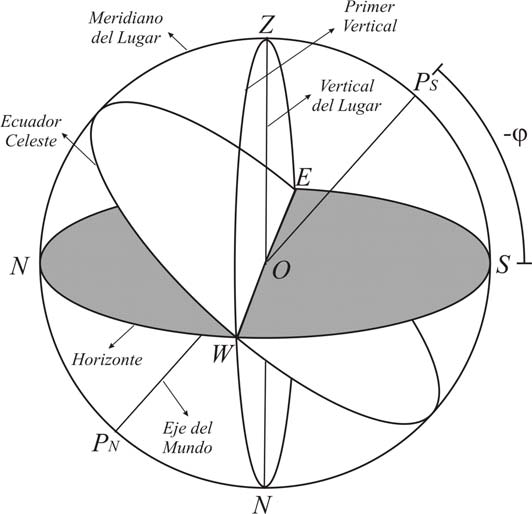
\includegraphics[scale=0.5]{esfera_celeste_lugar}
	\caption{Esfera celeste sobre un punto de la tierra}
	\label{fig:esfera_celeste_point_earth}
\end{figure}


\section{Sistemas de coordenadas} 

Los sistemas de coordenadas empleados, dependen del observador, existen varios sistemas de coordenadas astronómicos. En este apartado, solamente se verán dos, los cuales son los que se usan en este trabajo. Estos son las coordenadas horizontales, y las coordenadas ecuatoriales horarias. Sin embargo, cabe destacar que existe otro sistema de coordenadas ecuatoriales, denominadas coordenadas ecuatoriales absolutas, que no mencionamos, por tener que considerar otros conceptos, como eclíptica, y tiempo sidéreo, y además, la medida de estos. Además, cada sistema de coordenadas, considera un plano fundamental, sobre el cual se tomas medidas angulares, y estos planos definen los sistemas de referencia. 

\subsection{Sistema de referencia horizontal}

Este sistema es un sistema de coordenadas, con origen en el observador sobre un punto de la tierra. Su eje fundamental, es la esfera celeste, ubicada en la posición del observador. Sus ejes principales son la línea zenit – nadir, y el plano del horizonte. Este plano, en su corte, con el meridiano local, genera la línea norte—sur sobre el plano del horizonte. Este plano, además, si trazamos una perpendicular a la línea norte – sur por el centro de la esfera (posición del observador), tenemos los otros puntos, llamados este—oeste. 
En este sistema de coordenadas, se define un ángulo cero. Este punto, puede ser el norte o el sur sobre el plano del horizonte. A partir de él, dirigiéndonos hacia el este, lo tomamos en sentido positivo. Este ángulo se conoce con el nombre de “angulo de azimuth”. El cero que este en el norte o el sur, depende del tipo de materia que estemos analizando. En astronomía en general se toma el sur, y en navegación se toma el norte como cero. En nuestro trabajo consideramos el cero al norte, esto es asi, pues el software sobre el que se esta desarrollando asi lo indica en su manual. Cabe destacar que este ángulo, se denota con la letra Az o simplemente A.   
El otro ángulo es la altura. Una vez girado el ángulo de azimuth, este debe elevarse sobre el plano del horizonte, un cierto ángulo. Este ángulo se conoce con el nombre de “altura” o “elevación”. Esta altura ira entre 0 y 90º. En general se denota con la letra H. Además, sino se define la altura, se puede definir la “distancia zenital” que es z = 90º-H. A continuacion, se repite la imagen \ref{fig:mov_antena} para aclarar lo expuesto: 

\begin{figure}[ht!]
	\centering 
	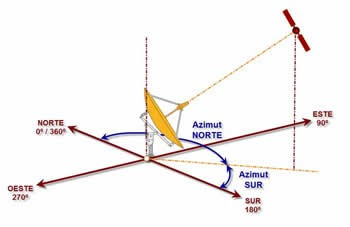
\includegraphics{movimiento_antena_hor}
	\caption{Coordenadas horizontales para realizar el apuntamiento de una antena. La antena que se pretende apuntar, posee este tipo de montura.}
\end{figure}

\subsection{Sistemas de coordenadas ecuatoriales} 

En este sistema, existen dos tipos: locales (o horarias) y celestes. En este tópico solo tratamos las coordenadas ecuatoriales locales, las celestes, requieren de otros conceptos, como tiempo sidéreo y plano de la eclíptica, y no se tratan en este informe.


El sistema de coordenadas ecuatoriales, basa sus ejes principales en el eje polar. Este eje polar, interseca el plano del horizonte en el origen de la esfera celeste. Perpendicular a esta línea, se traza un círculo máximo cortando a la esfera celeste, denominado ``ecuador celeste''. Todas las coordenadas son medidas a partir de estos ejes. Este tiene dos coordenadas: ángulo horario (simbolizado con la letra t), y ángulo de declinación denominado con la letra $\delta$.

 
El ángulo horario (t, H en la figura \ref{fig:coord_eq}), se mide desde la intersección del meridiano local, hasta el punto donde se encuentre el astro o satélite. Este ángulo en general se mide en horas, en sentido norte – este y oscila entre 0hs y 24hs. 
La declinación(D en la  \ref{fig:coord_eq}) se mide por el meridiano que pasa entre el polo elevado del horizonte (sur o norte, según la posición del observador en el planeta tierra), y el cruce con el ecuador. Este mide entre 0° y 90° positivos o negativos. Son negativos si se encuentran debajo del ecuador, y positivos si se encuentran por encima de él. La siguiente figura aclara lo expuesto en esta sección: 


\begin{figure}[ht!]
	\centering 
	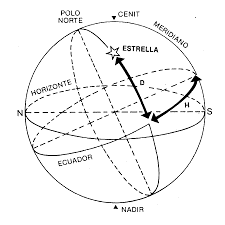
\includegraphics{coord_eq_local}
	\caption{Sistema de coordenadas ecuatoriales horarias. Estas se usan comunmente en telescopios de aficionados, debido a que solo requieren de un movimiento para seguir un astro.}
	\label{fig:coord_eq}
\end{figure}

\subsection{Transformación de coordenadas}

Los dos sistemas de coordenadas mostrados en este informe, usan dos coordenadas angulares para determinar la posición dentro del sistema de referencia utilizado. Estas posiciones, pueden transformarse de uno a otro. Esta cuenta, es la que debe realizarse cuando se usa el software stelarium dentro del microcontrolador. Por tal motivo, el único pasaje de coordenadas que mostramos en este inciso es la transformación de coordenadas ecuatoriales horarias a coordenadas horizontales. Cabe destacar, qué en este tipo de problemas, la latitud siempre es conocida. 
La transformación de coordenadas, implica trigonometría esférica. Se Hace uso de las fórmulas, del seno, coseno, y de los cinco elementos. 
Para empezar, se sabe que los datos conocidos son el ángulo horario, y la declinación, y la latitud del lugar. Con estos datos, y suponiendo el sur, como eje $0^\circ$ de las coordenadas horizontales y hacia el oeste. Con estos datos, se presenta el siguiente triangulo esférico mostrado en la figura \ref{fig:triang_esfer_ha}.  


\begin{figure}[ht!]
	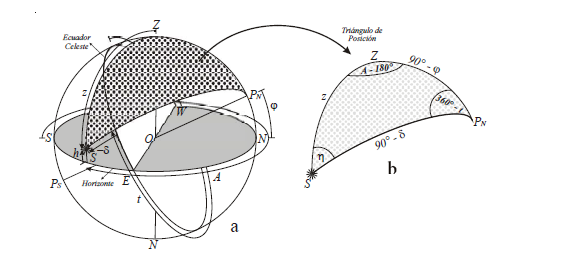
\includegraphics{transf_coord} 
	\caption{Transformación de coordenadas. Este triangulo recibe el nombre de triangulo de posición. Este triangulo depende de la posición del observador en la tierra}
	\label{fig:triang_esfer_ha}
\end{figure}

Cabe destacar, que la distancia entre el zenit y el polo norte, es 90$^\circ$ – $\phi$, si estamos ubicados en el polo norte, si estamos en el polo sur, esta distancia cambia a 90$^\circ$ + $\phi$. Con la declinación, ocurre que si estamos por debajo del ecuador, la distancia es 90-$\delta$ si la declinación esta en el hemisferio sur celeste, y si se encuentra en el polo norte, es positiva. Por este hecho, si el polo que esta dentro de nuestro horizonte visible es el polo sur, este ángulo es 90+$\delta$, donde delta va con su signo correspondiente. 

Del triángulo,se necesita el angulo A, y la altura h. La altura h, la se obtiene haciendo $z= 90^\circ – h$. El angulo $\eta$ utilizado en el gráfico, se denomina, \textbf{ángulo paraláctico}. 

Utilizando el teorema del coseno para triángulos esféricos: 
\begin{equation}
	\begin{split}
	\cos(z)  & = \cos(90^\circ -\delta)\cos(90^\circ -\phi) + \sin(90^\circ -\phi) \sin(90^\circ -\delta)\cos(360^\circ -t)  \\
	\cos(z)  & = \sin(\delta)\sin(\phi) + \cos(\phi) \cos(\delta)\cos(t)  
	\end{split}
\end{equation}

Con esto, se obtiene el ángulo $z$, dado que $z= 90 -h \rightarrow cos(90-h)=cos(h)$, entonces se tiene que:
\begin{equation}
	\cos(h) = \sin(\delta)\sin(\phi)+ \cos(\phi)\cos(\delta)\cos(t) 
\end{equation} 
Si se usa la fórmula de los cinco elementos, para el ángulo $A$, se tiene que 

\begin{multline}
	\cos(z)\sin(180^\circ-A) =\sin(z)\cos(A-180^\circ) = \cos(90^\circ - \phi)\sin(90^\circ - \delta) -\cos(90^\circ - \delta)\sin(90^\circ - \phi)\cos(360^\circ - t) 
\end{multline}

Con lo cual, se han obtenido dos ecuaciones para resolver el angulo de Azimut, y el de altura. Con esto, no nos alcanza para resolver el sistema, ya que la función inversa $\arccos(x)$ esta definida para $x$ entre $[-\pi/2 \pi/2]$.Por este motivo, se requiere de otra ecuación, que nos brinde el signo de $\cos(A)$, y luego realizando el coseno inverso, obtenemos el ángulo total. Para obtener el signo, se basa en el uso del teorema del seno esférico. Realizando esto, obtenemos la siguiente ecuación:  

\begin{equation}
	\begin{split}
		\frac{\sin(180^\circ-A)}{\sin(90^\circ-\delta)} &= \frac{\sin(360^\circ-t)}{\sin(z)} \\ 
		\sin(A)\sin(z) &= \sin(t)\cos(\delta) 
	\end{split}
\end{equation}

En resumen, las ecuaciones para realizar la transformación de coordenadas: 

\begin{equation} \label{eq:law_transform_coordinates}
	\begin{cases} 
		\cos(z) = \sin(\delta)\sin(\phi) + \cos(\phi)\cos(\delta)\cos(t) \\ 
		\sin(z)\cos(A) = -\cos(\phi)\sin(\delta) + \cos(\delta)\sin(\phi)\cos(t) \\	
		\sin(A)\sin(z) = \cos(\delta) \sin(t) 
	\end{cases}  
\end{equation}

De la primera ecuación, obtenemos el valor de $\cos(z)$, tomando la función inversa, obtenemos el valor de $z$. Se realiza, $z = 90 -h$ y se obtiene el ángulo de altura. 

Con el valor de $z$, se introduce, en la segunda ecuación, y se obtiene el signo de $\cos(A)$. La función inversa del coseno, devuelve valores entre 0 y 180°. Debido al sistema de coordenadas que se ha seleccionado para medir los ángulos(sistema horizontal), si el $\cos(A)<0$, se debe sumarle 90° al A encontrado. Si el $\cos(A)$, es positivo, se debe resolver, de la manera usual. Esto es, si esta entre 0 y 90°, corresponde este ángulo, y si esta por encima de 90°, corresponde, restarle 360°. A continuación, se deja una tabla, con los resultados de esta sección. 

\begin{table}[ht!]
	\centering
	\begin{tabular}{|c|c|}
		\hline
		Signo del coseno A & Ángulo de azimut  \\
		\hline 
		$\cos(A)>0$ y  $0^\circ<A<90^\circ$ & Az \\
		\hline
		$\cos(A)>0$ y  $90^\circ<A<180^\circ$ & $360^\circ - Az$ \\
		\hline
		$\cos(A)<0$ y  &  $90^\circ + Az$ \\
        \hline
	\end{tabular}
	\caption{Resumen del valor del ángulo de azimut en base al signo de $\cos(A)$}
\end{table}

Cabe recordar, que esta deducción se realiza para poder realizar la cuenta dentro del microprocesador Arduino, y luego mover los motores hacia esa posición. Se debe tomar en cuenta, que el software Stellarium, brinda las coordenadas en el sistema ecuatorial, y se deben transformar al sistema horizontal dentro del microcontrolador. 

\section{Coordenadas Software Stellarium}

El programa stellarium, utiliza coordenadas ecuatoriales absolutas. Estas coordenadas, son iguales a las ya vistas, excepto que el cero, se toma sobre un punto fijo, denominado ``punto vernal''.Este punto, define el tiempo sidéreo local. Para realizar esta transformación, se debe considerar la implementación de una base de tiempo sidéreo. Este planteo, escapa el alcance general del proyecto, ya que el agregado de esta base de tiempo, demanda aproximadamente un mes más de proyecto, y no se pueden cumplir con el cronograma previsto. Por este motivo, se plantea este capítulo, donde se brindan las ecuaciones, y queda como trabajo futuro la implementación de la transformación de coordenadas. Los pasos a seguir para la transformación de coordenadas dentro del microcontrolador son los siguientes: 
\begin{itemize}
	\item Obtener Hora sidérea Local 
	\item Realizar la implementación del sistema de ecuaciones \ref{eq:law_transform_coordinates}
	\item Transfomación de coordenadas obtenidas al sistema HMS(hora-minuto-segundo), para realizar la validación de los datos con el mismo software. 
	\item Prueba y validación de los datos mediante algún mecanismo visual(display, puerto serie, etc) a definir. 
\end{itemize} 

\section{Conclusiones}

En este trabajo, se muestra la complejidad y dificultad de realizar un apuntamiento hacia un objeto celeste. Este trabajo, solo muestra algunos resultados, de todos los que se han investigado, para llegar a la solución de la transformación de coordenadas. Este tópico, se considera una de las partes fundamentales para el apuntado, ya que de ella dependen los movimientos de los motores. Además, en este trabajo, no se han tenido en cuenta errores debido a movimientos de la tierra(en especial: nutación y precesión), y otros efectos, como pueden ser el paralaje y la aberración, o la forma semiesférica de la tierra, y el geoide de referencia. Sin incluir, que se han dejado de lado conceptos como tiempo sidéreo y plano de la eclíptica. Estos tópicos nombrados anteriormente, deberían tenerse en cuenta, si el apuntamiento debe ser preciso, pues los movimientos de nutación y precesión, tienen el efecto de cambiar los ángulos de las estrellas en el cielo, y pueden perturbar las orbitas de los satélites, además, cambian el punto sidéreo referenciado como cero.
Los puntos que se explican en el tópico transformación de coordenadas son los que se deben programar dentro del microcontrolador, para que pueda apuntar a una estrella con el software Stellarium, en especial la ecuación de transformación. En este trabajo, no se ha implementado debido a que no cumple con los tiempos previstos por el proyecto. 


